\chapter{Benchmarking and Performance Evaluation}
\label{chapter:experiments}

Technical debt can have direct implications on the performance and failure rate of a system.

The goal of this Chapter is to quantify the performance of various common operations performed by users in Tribler. We will perform a number of experiments and for each experiment, we will present and discuss the observed results. The underlying reason for this experiment is twofold: on the one hand, we would like to show that the performance of the system did not degrade with to unacceptable extent. On the other hand, we use the performance measurements to identify possible issues that is classified as future work.

\section{Environment specifications}
The experiments performed in this Chapter using the Tribler core are executed on a virtual private server. An important condition is to stay as close as possible to the specifications of a machine that an actual user could be using. The virtual server has 8GB of memory and 1 processor with 4 cores (where each core has a clock speed of 2.5GHz). The used operation system is Ubuntu 15.10. The experiments are not executed in an isolated, artificial environment but instead in the wild, using the deployed Dispersy network. While the obtained results may be different between users, this setup can be used to get insight in the performance of Tribler from a user's perspective.\\\\
If not stated otherwise, the default values of the Tribler configuration file are used. These default values can be found in the `defaults.py` file in the source code directory of Tribler\footnote{https://github.com/Tribler/tribler/blob/devel/Tribler/Core/defaults.py}. In this configuration file, all communities, except for \emph{BarterCast}, are joined.\\\\
Some of the experiments are specified by the usage of a scenario file. In such a scenario file each line specifies a specific command of a peer at a specific point in time into the experiment. Our framework to run the experiments, Gumby, contains code to read scenario files, interprets the commands to be executed and to schedule them on the reactor thread. Several utility methods have been implemented to gather and write statistics to files in a processable and readable format that can be parsed by visualization tools such as \emph{R}. The usage of scenario files is already adopted in various Dispersy experiments, mainly in our \emph{AllChannel} experiment that runs on the DAS5 supercomputer. We extended the usability of this approach to run a Tribler client and we improved the framework by adding various commands to support operations as conducted in the performed experiments in this Section. An overview of the implemented commands can be found in Appendix \ref{appendix:gumby-scenario-commands}. The flexibility of these scenario files gives the next generation of Tribler developers a robust framework to use when conducting performance analysis, scientific research and benchmarking.

\section{Profiling Tribler on low-end devices}
\label{sec:profiling_tribler_lowend}
The addition of a REST API allows developers an option to run and control Tribler remotely using the HTTP API. For instance, one can run Tribler on a low-end, cheap devices such as a Raspberry Pi. Android is another example of a device that can run Tribler and during the last years, various research have been conducted to explore the possibilities of Tribler on Android devices\cite{sabee2014tribler}\cite{de2014android}. Executing and profiling Tribler on a low-end device with limited resources can yield much information about bottlenecks that might not be directly visible when running Tribler on a desktop or supercomputer.\\\\
The experiments described in this Section are all executed on a Raspberry Pi, third generation with 1GB LPDDR2 ram, 4× ARM Cortex-A53, 1.2GHz CPU and 16GB storage on a microSD card. The used operating system is Raspbian, a system specifically designed for the Raspberry Pi and derived from the desktop Debian operating system.\\\\
Regular usage of Tribler on the Raspberry Pi using the REST API has us suspected that the Raspberry Pi is under heavy load when running Tribler. Monitoring the process for a while using the \emph{top} tool, reveals that the CPU usage is often around 100\%, completely filling up one CPU core. To get a detailed breakdown of execution time per method in the code base, the Yappi profiler has been used to gather statistics about the runtime of methods. This profiler has been integrated in the \emph{twistd} plugin and can be started together with Tribler by passing a flag. The output generated by the profiler is a \emph{callgrind} file that should be loaded and analysed by third party software. The breakdown of a 20-minute run is visible in Figure \ref{fig:yappi_breakdown}. This breakdown is generated using \emph{QCacheGrind}, a \emph{callgrind} file visualizer. In this experiment, we start with a clean state directory which is equivalent to the first boot of Tribler.

\begin{figure}[!h]
	\centering
	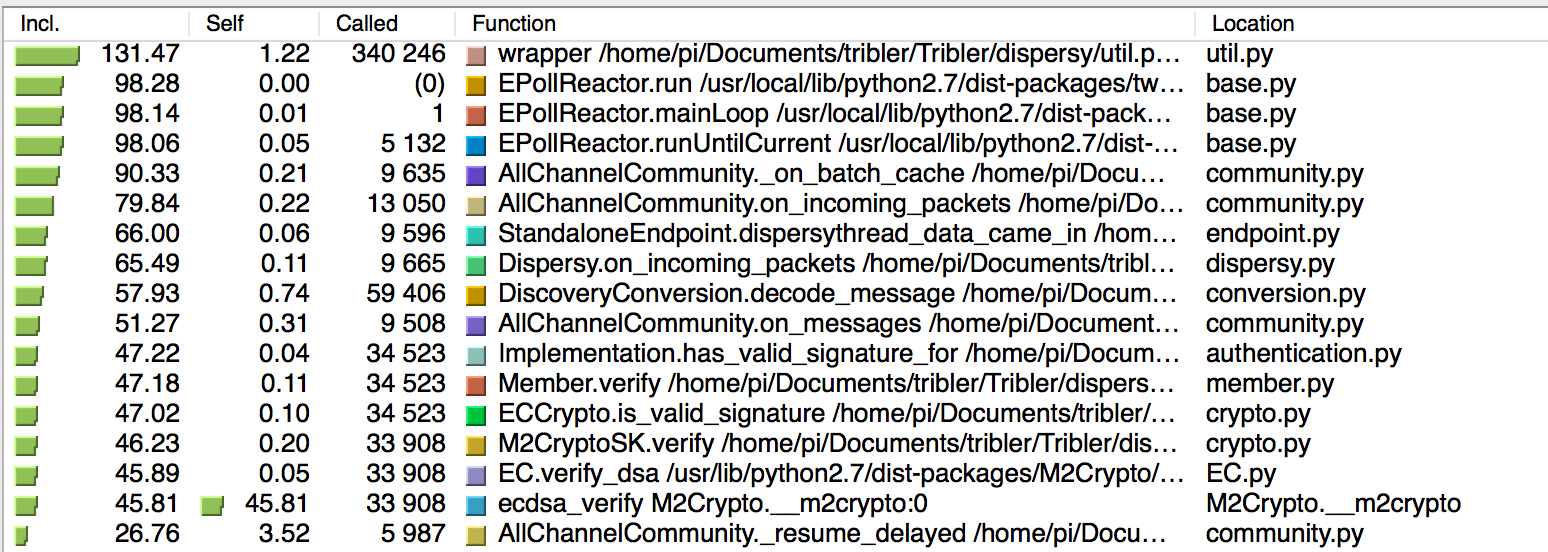
\includegraphics[width=0.9\columnwidth]{images/experiments/yappi_breakdown}
	\caption{The breakdown of a 20-minute run of Tribler on the Raspberry Pi.}
	\label{fig:yappi_breakdown}
\end{figure}

The file created by the Yappi profiler provides a detailed overview of the execution time of methods and can be used as a tool to detect performance bottlenecks in the system. Referring to Figure \ref{fig:yappi_breakdown}, the column \emph{Incl.} denotes the inclusive cost of the function, in other words, the execution time of function itself and all the functions it calls. The column \emph{self} denotes only the execution time of the function itself, without considering callees. The other columns are self-explanatory and can be used as reference to the location of the respective function in the source code.\\\\
If we analyse the breakdown, it is clear that Dispersy has a big impact on the performance of Tribler when running on the Raspberry Pi. The \emph{ecdsa\_verify} method (second method from the bottom) is dominating the runtime of Tribler: 45.81\% of the time Tribler is running, is spent inside this method. This specific method verifies the signature of an incoming Dispersy message and is invoked every time a signed message is received. Disabling cryptographic verification of incoming messages should improve the situation, however, this is a trade-off between security and performance: by not verifying incoming messages, fake messages by an adversary can be forged and are accepted in such as system.\\\\
To verify whether the responsiveness of Tribler improves when we disable cryptographic verification of incoming messages, we measure the CPU usage of two runs. Both runs start with a non-existing Tribler state directory and have a duration of ten minutes. In the first run, we are using the default configuration of Tribler, like in most of the other experiments described in this Chapter. In the second run, we disable verification of incoming messages. The CPU utilization over time of the two runs are displayed in Figure \ref{fig:raspi_cpu_usage}.\\\\

\begin{figure}[!h]
	\centering
	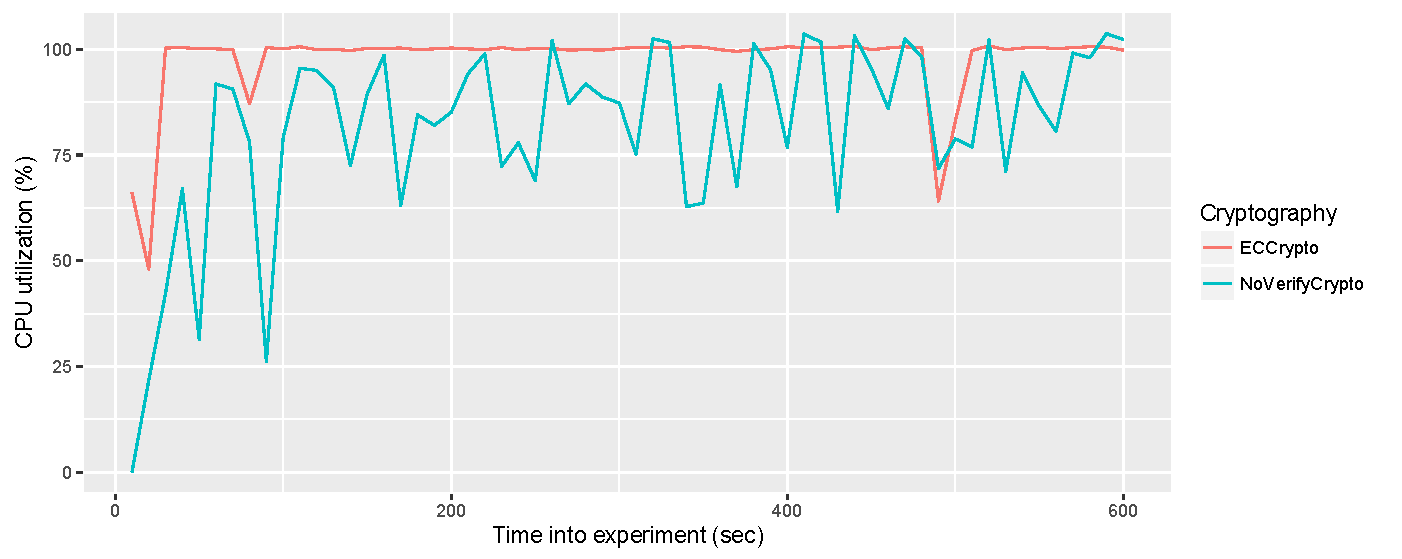
\includegraphics[width=1.0\columnwidth]{images/experiments/raspi_cpu_usage}
	\caption{The CPU utilization of one core on a Raspberry Pi device when running Tribler with different cryptographic policies.}
	\label{fig:raspi_cpu_usage}
\end{figure}

In Figure \ref{fig:raspi_cpu_usage}, some occurrences are visible where the CPU usage appears to be slightly over 100\%. This is explained by the fact that some of the underlying code is designed to run on multiple processors. While the threading model of Tribler is limited to a single core, the Python interpreter might execute code on additional cores to improve performance. In the run where we enable all components of the system, the CPU usage is often 100\%. When verification of Dispersy messages is disabled, we observe a somewhat lower CPU usage but overall, this utilization is still high. Unfortunately, disabling incoming message verification is clearly not enough to guarantee a more usable and responsive system.\\\\
To detect other performance bottlenecks, we sort the report generated by the Yappi profiler on the \emph{Self} column to get insight in methods that are taking a long time to complete. This is visible in Figure \ref{fig:yappi_breakdown_self}. An interesting observation here is that the Python built-in \emph{all} method takes up a significant amount of time (6.13\% of the runtime). The \emph{all} method takes an iterable object and returns \emph{true} if all objects of this collections are true. Both the \emph{all} method and \emph{zip} method (also visible in Figure \ref{fig:yappi_breakdown_self}) is used in the \emph{\_resume\_delayed} method, indicating that this method might causing performance issues. Since further analysis of this method requires more knowledge of Dispersy, optimization of this bottleneck is considered future work and described in GitHub issue 505\footnote{https://github.com/Tribler/dispersy/issues/505}.\\\\

\begin{figure}[!h]
	\centering
	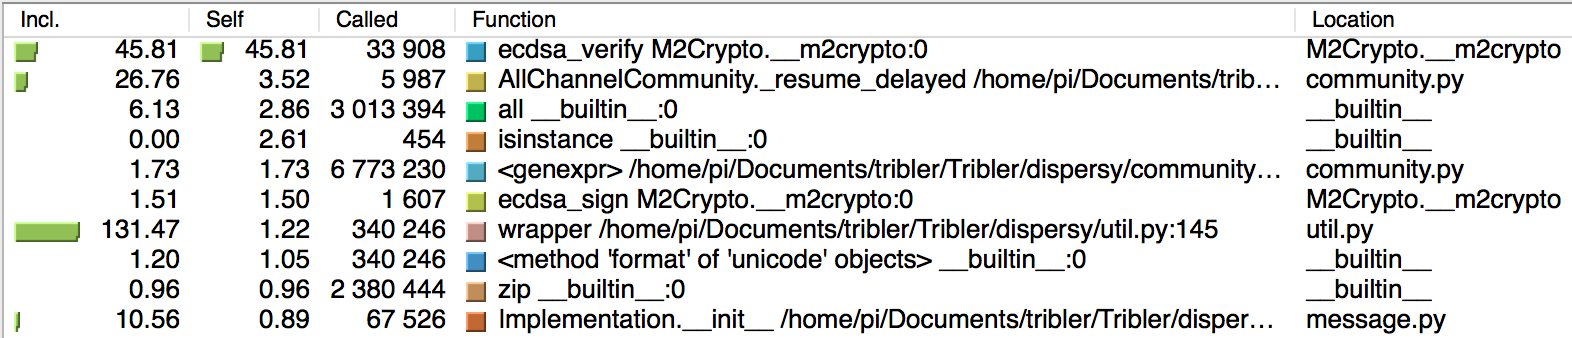
\includegraphics[width=0.9\columnwidth]{images/experiments/yappi_breakdown_self}
	\caption{The breakdown of a 20-minute run of Tribler on the Raspberry Pi, sorted on the \emph{Self} column.}
	\label{fig:yappi_breakdown_self}
\end{figure}

In this Section, we demonstrated how adequate usage the Yappi profiler can lead to the detection of bottlenecks in the system. Integration in the twistd plugin makes it convenient for developers to run and analyse Tribler sessions under different circumstances.

\section{Performance of the REST API}
The responsiveness of the REST API is directly influencing the user experience. If the response times of API calls is high, users of Tribler have to wait longer before their data is available and visible. For this reason, we wish to make the API serve requests as fast as possible. The experiments to assess the performance of the API will particularly focus on latency of requests, however, some other statistics will be considered such as average request time, standard deviation of the response times and observed bandwidth. These statistics will help us to get more insights in the performance of the REST API.\\\\
We make use of Apache JMeter\cite{jmeter2010apache} that is used to perform HTTP requests to Tribler and to gather and process performance statistics. The application allows to simulate a realistic user load, however, in this experiment we will limit the load to one user that performs a request to Tribler with a fixed interval. This request will be targeted to a specific endpoint in the API: \emph{/channels/discovered}. This exact call happens when users are pressing the \emph{discover} menu button in the new Qt GUI and the response of the request contains a JSON-encoded dictionary of all discovered channels that Tribler has discovered. As a consequence, the returned response can be rather large, especially if Tribler has been running for a long time and has discovered many channels (in our experiments, the average response size is around 613KB). When Tribler is processing the request, a database lookup is performed to fetch all channels that are stored.\\\\
We perform various experiments with different intervals between requests made and a fixed total amount of 500 requests. First, we perform the experiment with one request every second and we expect that the system should easily be able to hand this load and serve these requests in a timely matter. Next, the frequency of requests is increased to respectively 2, 5, 10 and 15 requests per second. These numbers are determined emperically and are based on the average request time, which appears to be several hundred milliseconds. Each experiment is started around five seconds after Tribler has started where we are using a pre-filled database with around 100.000 discovered torrents and 1.200 channels. A summary of the results of these experiments are visible in Table \ref{table:performance-api-results}.\\

\begin{table}[]
	\centering
	\begin{tabular}{|l|l|l|l|l|l|l|}
		\hline
		\textbf{Requests/sec} & \textbf{Avg. (ms)} & \textbf{Std. dev (ms)} & \textbf{Median (ms)} & \textbf{Min. (ms)} & \textbf{Max. (ms)} & \textbf{KB/S} \\ \hline
		\emph{1} & 241 & 476.34 & 76 & 56 & 4246 & 585.58\\ \hline
		\emph{2} & 170 & 327.86 & 68 & 58 & 3394 & 1127.04\\ \hline
		\emph{5} & 123 & 210.23 & 60 & 52 & 2082 & 2538.36\\ \hline
		\emph{10} & 115 & 238.72 & 60 & 50 & 2450 & 4120.70\\ \hline
		\emph{15} & 182 & 497.61 & 68 & 52 & 4937 & 3296.45\\ \hline
	\end{tabular}
	\caption{A summary of the experimental results when measuring the performance of the REST API.}
	\label{table:performance-api-results}
\end{table}

The most interesting observation in this Table is that it appears that requests are completed faster if we are performing requests at a faster rate, indicating that Tribler is able to handle the incoming requests well. This is surprising since one would expect the results to be the other way around: when the frequency of requests is increased, the average request time increases since Tribler might receive incoming requests while the previous incoming request is still being processed. The observed result is most likely due to caching of data which might be performed by the underlying database engine.\\\\
The standard deviation of the request times in Table \ref{table:performance-api-results} is rather large compared to the average request time. We suspect that this can be explained by the fact that Tribler is performing many different operations that are influencing the request times. In particular, we think that the reactor thread is busy with processing other calls that are scheduled earlier, causing the API calls to be processed later. To verify this, we ran the experiment again where we enable Dispersy, the component responsible for many calls in the reactor (as described in Section \ref{sec:profiling_tribler_lowend}). We perform five requests per second and 500 requests in total for this experiment. The observed results of are illustrated in Figure \ref{fig:api-performance} (the left plot corresponds to the 5 requests/sec row in Table \ref{table:performance-api-results}). In the left plot, the response times of the performed requests with a regular Tribler session is displayed whereas in the right plot, we display the response times of the run where we disable Dispersy. Note the different scale on the vertical axis, indicating that the requests performed when Dispersy is disabled, are substantially faster. Indeed, the average request time of the right plot is 48 ms, significantly lower than the average of the response times when Dispersy is enabled, namely 123 ms. While both graphs are producing a spiky pattern, the standard deviation of the right plot is 5.73 ms and the standard deviation in the left plot is 210.23 ms. We conclude that the variation in response times is much lower in the right plot and that most likely DIspersy is producing a big amount of work for the reactor thread, introducing considerable amounts of latency when performing API requests.\\

\begin{figure}[h!]
	\centering
	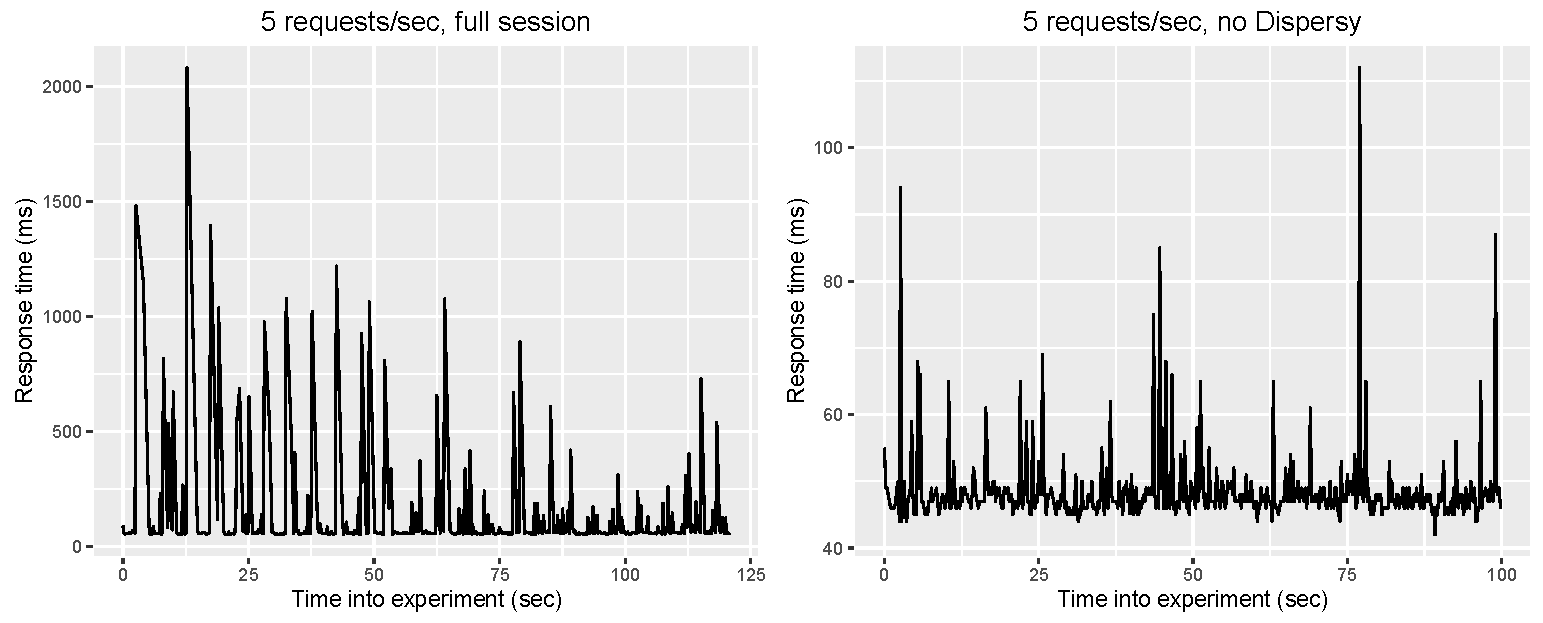
\includegraphics[width=1.0\columnwidth]{images/experiments/request_times_comparison}
	\caption{The response times of API requests, both within a full session and in a session where Dispersy has been disabled.}
	\label{fig:api-performance}
\end{figure}

We identified a key issue here: the latency of methods to be processed in the Twisted reactor is high, causing the processing of incoming requests to be delayed. This does not only hold for the REST API: we can conclude the same for Dispersy and the tunnel community where possibly many incoming connections have to be served. The most important part of the solution is to make sure that there are no big blocking calls scheduled on the reactor thread that are taking a long time to complete. When a method call with a high runtime is executed on the reactor thread, Tribler is unable to process other events during that period, leading to an unresponsive system. Ongoing work is focussed on making the disk operations on the reactor thread non-blocking and as a consequence, reducing the latency of event processing and improving the responsiveness of the system in general.\\\\
Table \ref{table:performance-api-results} gives us another interesting observation, namely that we it appears that the bandwidth is reducing as the number of requests per second increases. This is in particular clear if we plot the theoretical maximum bandwidth against the observed bandwidth during the experiments, see Figure \ref{fig:api-bandwidth-performance}. In this Figure, we presented both the obtained bandwidth for a run using the regular Tribler session and a session where Dispersy has been disabled. We assume that each request contains 613KB of data in the response. The theoretical bandwidth is calculated as $ b = 613* n $ where $ n $ is the number of requests per second and $ b $ is the theoretical maximum bandwidth in KB/s. In practice, we will never reach this theoretical bandwidth since some time is required to create the connection and to process the response data in Tribler which we do not consider in our simple bandwidth model. We still notice that the obtained bandwidth is somewhat becoming constant, indicating that the bandwidth we can obtain is limited. This picture clearly shows the impact of a running Dispersy on the bandwidth. Whereas we almost obtain the theoretical output when we disable Dispersy, the gap between the theoretical and observed bandwidth becomes bigger in the run where we use a full session. When performing fifteen requests per second, the bandwidth even decreases, possibly due to the high system load the concurrent requests are causing.

\begin{figure}[h!]
	\centering
	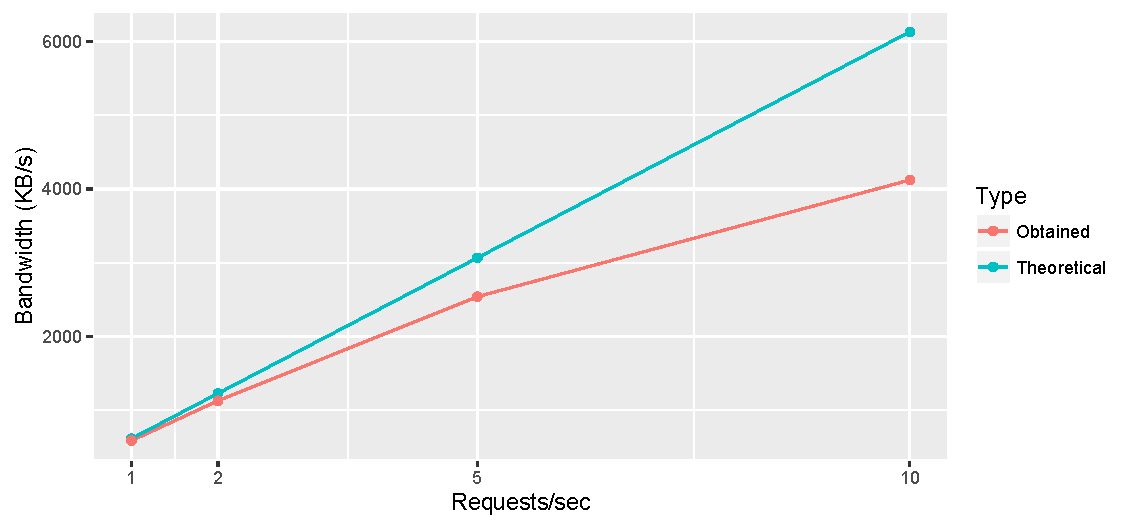
\includegraphics[width=1.0\columnwidth]{images/experiments/api_bandwidth_performance}
	\caption{The maximum theoretical bandwidth compared to the obtained bandwidth (using a full Tribler session and disabled Dispersy) in the experiments.}
	\label{fig:api-bandwidth-performance}
\end{figure}

\section{Start-up experience}
The first interaction that users have with Tribler, is the process of booting the software. During this boot process, various operations are performed:
\begin{itemize}
	\item The Tribler state directory is created and initialized with necessary files such as the Dispersy key pair and configuration files.
	\item A connection to the SQLite database is opened and initialized. If this database does not exist, it will be created first.
	\item Dispersy is started and the enabled communities in the configuration file are loaded.
	\item Various Tribler components are created, including the video streaming server, the REST API, the remote torrent handler and the \emph{leveldb} store.
\end{itemize}
The start-up process of the Tribler core proceeds sequentially and no parallel operations are implemented to speed up the process. Depending on the number of enabled components, the start-up time might vary.\\\\
To analyse the start-up time, Tribler is started 50 times. The experiments are performed several times where in one experiment the software is started for the first time, with no prior existing state directory. In these runs, a state directory is created and the required files are initialized. In another experiment, a database containing just over 100.000 torrents is used. This database is the result of running Tribler idle for several hours, after subscribing to some popular channels to fetch as much torrents as possible. The filled Tribler database comes in conjunction with a filled Dispersy database. In both scenarios, there are no active downloads. The experiment starts when the \emph{start} method of the \emph{Session} object is called and ends when the notification that Tribler has started, is observed. During the span of this thesis, there have been various changes to the start-up procedure of Tribler where some code has been modified. Since we wish to make sure that our modifications do not significantly decrease the start-up speed, we make a comparison between the code in November '15 and July '16. The results are displayed in Figure \ref{fig:startup_experiment}, where for each commit we compare, we present an ECDF with the boot time on the horizontal axis and within each plot, the distribution of boot times from a clean and pre-filled state.\\

\begin{figure}[!h]
	\centering
	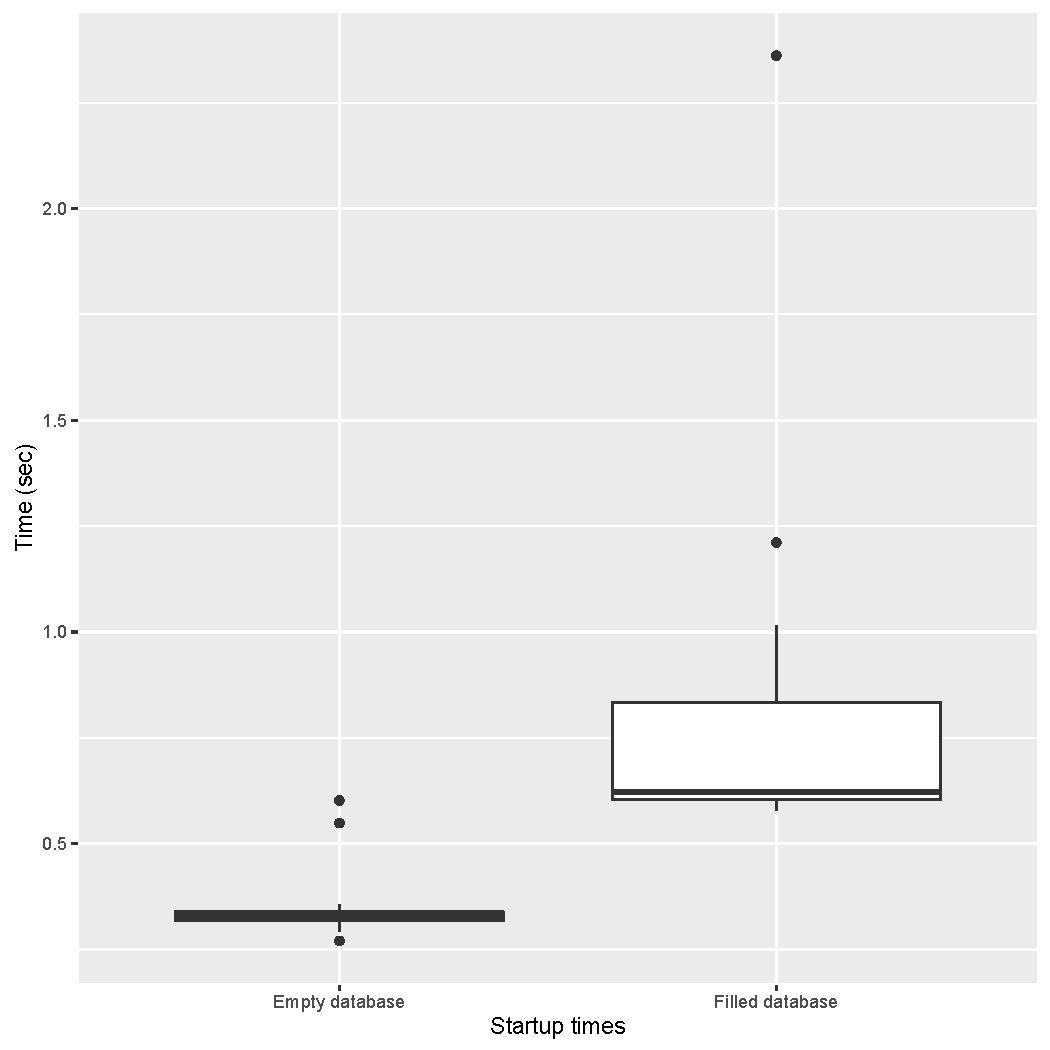
\includegraphics[width=1.0\columnwidth]{images/experiments/startup}
	\caption{The boot time of Tribler from a clean and pre-filled state using the code base in November '15 and July '16.}
	\label{fig:startup_experiment}
\end{figure}

In both plots, It is clear that magnitudes of the Tribler and Dispersy databases have impact on the time for Tribler to completely start. However, this impact is relatively minor since Tribler still starts well within a second. We think that this statistic justifies removal of the splash screen that is shown in the old user interface. The relatively short time the splash screen would be visible in the new interface is so short that users would not even be able to read and interpret the content of the splash screen. In contrast to the old user interface, the new interface starts Tribler and shows a loading screen after the interface has started. However, users are able to already browse through other tabs such as their downloads and discovered channels.\\\\
Whereas the boot times of the runs performed with the November '15 code are very constant, we notice a variation in the runs with the code base from July '16, indicating that there is some component that has a high variation in initialization time. Further analysis learns us that this variation can be addressed to Dispersy, possibly caused the boot procedure of one of the communities. However, further analysis of the boot time of Dispersy is outside the scope of this thesis work.

\section{Remote Content Search}
\label{sec:remote-content-search-experiment}
We wish to serve relevant information to users as fast as possible. To help users search for content they like, a remote keyword search has been implemented, where users can search for torrents and channels. Channel results are fetched by a query in the \emph{AllChannel} community whereas torrent results are retrieved by a query in the \emph{search} community.\\\\
To verify the speed of the remote torrent search, various experiments are conducted. We are using a list of 100 terms that are guaranteed to have matches in the network. Each search query is executed when there are at least 20 connected peers in the \emph{SearchCommunity}. The time-out period of the remote search is 60 seconds, indicating that search results that are coming in after this period are not regarded. This experiment has a particular focus on two statistics: the time until the first remote torrent search results comes in and the turnaround time of the search request, indicating the time until the last request comes in. We should note that users performing a remote search might see results earlier since a search query in the local database is performed in parallel. The results are visible in Figure \ref{fig:remote_search}.\\\\
Overall, the remote torrent search as implemented in Tribler is very fast and performs well. For every search query performed, we had at least one incoming result and on average, 61 search results are returned for each query where the first incoming torrent result takes 0.26 seconds to arrive. As we see in Figure \ref{fig:remote_search}, over 90\% of the first remote search results are available to the user within a second. During our experiment, we always have the first incoming torrent result within 3.5 seconds. The other graph shows the turnaround time of the request, indicating the time until the last response within our time-out period. On average, it takes 2.1 seconds for all torrent search results to arrive. In the plot, we see that in over 90\% of the search queries, we have all results within 10 seconds.\\

\begin{figure}[!h]
	\centering
	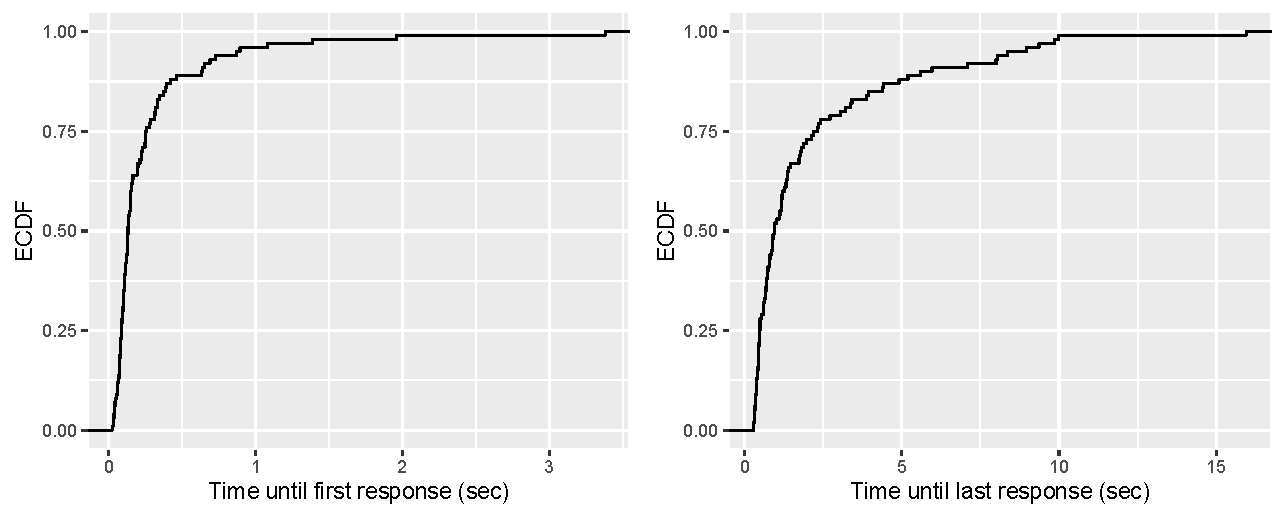
\includegraphics[width=1.0\columnwidth]{images/experiments/cdf_remote_search}
	\caption{The performance of remote content search, expressed in the time until the first response and time until last response.}
	\label{fig:remote_search}
\end{figure}

The same experiment has been performed in 2009 by Nitin et al. where 332 remote search queries have been performed, see Figure \ref{fig:nitin_remote_search} where the time until the first response from any remote peer in the network is measured. The graph makes a comparison before and after a significant improvement to the I/O mechanism, causing messages to be exchanged faster. The observed average time until first response in 2009 is 0.81 seconds whereas our observed average time is 0.26 seconds.

\begin{figure}[!h]
	\centering
	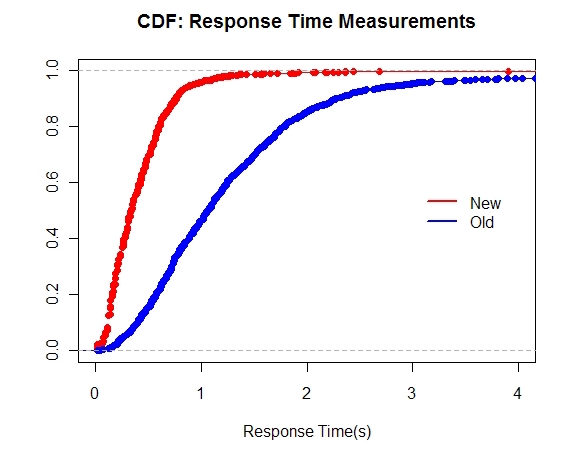
\includegraphics[width=0.7\columnwidth]{images/experiments/nitin_remote_search}
	\caption{The performance of remote content search, performed by Nitin et al. in 2009. The new remote search had an improved I/O mechanism, causing messages to be exchanged faster.}
	\label{fig:nitin_remote_search}
\end{figure}

\section{Local Content Search}
\label{sec:local-content-search}
In the previous Section, we demonstrated and elaborated the performance of the remote content search mechanism. Now, we will shift the focus to performance measurements of a local content search, which is considered more trivial than the remote search counterpart where network communication is required. In particular, our goal is to quantify the performance gain or loss when switching to the new relevance ranking algorithm, as described in Chapter \ref{sec:relevance-ranking-algorithm}.\\\\
The setup of the experiment is as follows: a database with just over 100.000 torrents is used. Around ten seconds after starting Tribler, we perform a local \emph{torrent} search every second and we do this for 1.000 random keywords that are guaranteed to match at least one torrent in our database. We will measure both the time spent by the database lookup and the time it takes for the data to be post-processed after being fetched from the database. In the old relevance ranking algorithm, this post-processing step involves determining the associated channels for each torrent result. This experiment is performed for the old ranking algorithm that uses the Full Text Search 3 (FTS3) engine and the new ranking algorithm that uses the more recent FTS4 engine. According to the SQLite documentation, FTS3 and FTS4 are nearly identical, however, FTS4 contains an optimization where results are returned faster when performing searches with keywords that are common in the database. The results are visible in Figure \ref{fig:local-search-fts3-fts4}, presented in two ECDF plots.\\

\begin{figure}[h!]
	\centering
	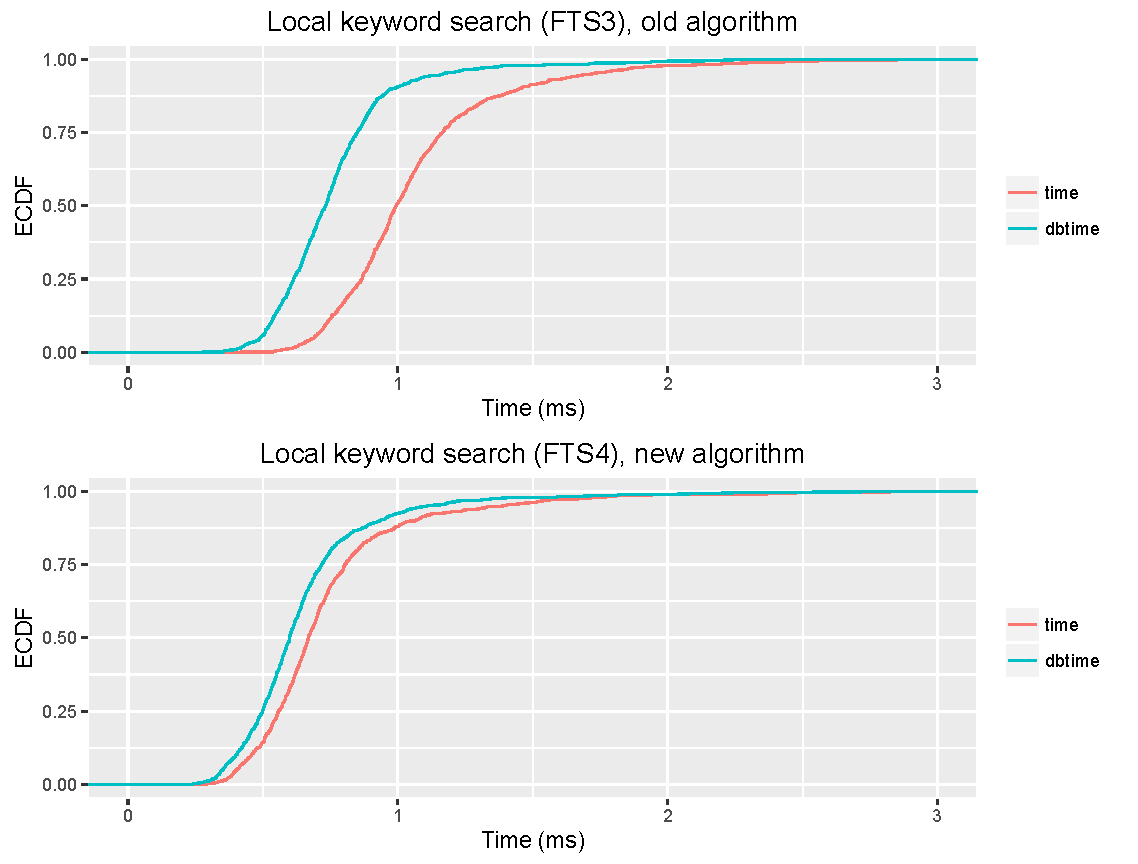
\includegraphics[width=1.0\columnwidth]{images/experiments/local_search_fts3_fts4}
	\caption{A comparison of the performance of local keyword searches between the old ranking algorithm with the FTS3 engine and the new ranking algorithm utilizing the FTS4 engine.}
	\label{fig:local-search-fts3-fts4}
\end{figure}

Local content search is very fast, delivering results in several milliseconds and low priority should be given to performance engineering on the local content search engine. We see that the two lines in the FTS3 and FTS4 graphs have moved closer to each other which means that the speed of post-processing of torrent results has increased. This is in line with our expectations since the new relevance ranking algorithm should be less computationally expensive than the old one. In addition, the new algorithm takes less factors in considering, for instance, the swarm health of the torrent. The increase in performance from FTS3 to FTS4 is visible but not significant.\\\\
In 2009, Nitin et al. performed the same experiment where they used a database filled with 50.000 torrents. Their generated ECDF is displayed in Figure \ref{fig:local-search-nitin}. We notice that the current performance of local search in our experiment is dramatically better than the performance obtained during the 2009 experiment. This can be explained by the fact that Tribler used a custom inverted index implementation when the experiment in 2009 was conducted. An inverted index is an index data structure where a mapping is stored from words to their location in the database and is used on a large scale by search engines, including the FTS engine of SQLite. By utilizing this mapping when performing a full text search, we can get results in constant time. However, there is a slight overhead for maintaining and building the inverted index when new entries are added to the database, also impacting the size of the database disk file. The built-in FTS engine of SQLite is optimized to a large extent and clearly offers a higher performance than a custom implementation.

\begin{figure}[h!]
	\centering
	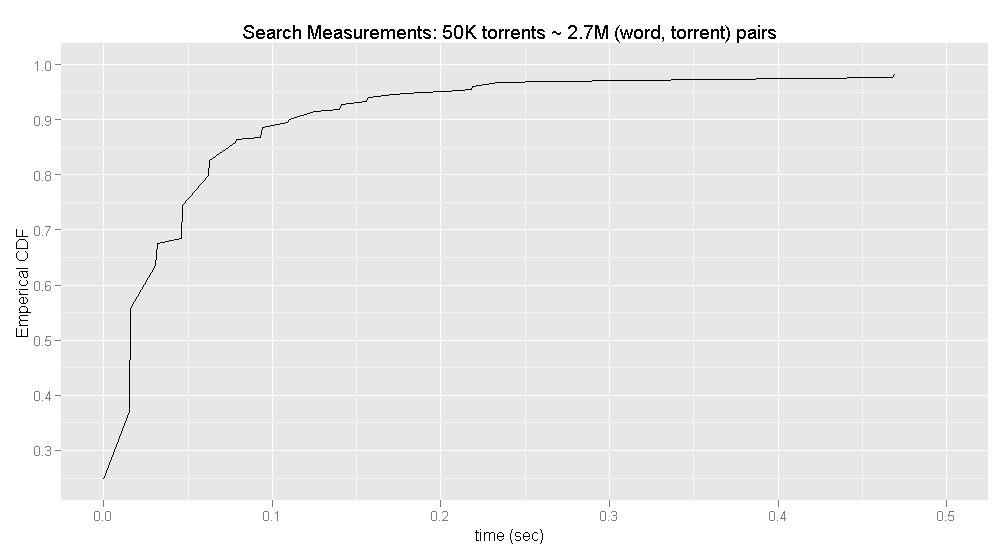
\includegraphics[width=1.0\columnwidth]{images/experiments/nitin_local_search}
	\caption{The performance of a local database query as verified by Nitin et al. in 2009.}
	\label{fig:local-search-nitin}
\end{figure}

\section{Video streaming}
The embedded video player in Tribler allows users to watch a video that is being downloaded and is explained in more detail in Chapter \ref{subsubsec:video-server}. Video playback has been available since Tribler 4.0. It is based on VLC and offers support for seeking so the user can jump to a specified offset in the video. Video downloads have a special Video On Demand (VOD) mode which means that the \emph{libtorrent} library piece picking mechanism uses a linear policy mode. In this mode, pieces are downloaded in a timely matter. When the user seeks to a position in the video, the prioritization of the pieces are modified, giving priority to pieces just after the specified seek position. Users also have the possibility to use an external video player that support playback of HTTP video streams.\\\\
The bytes are streamed to a VLC client using a HTTP stream. When Tribler starts, a HTTP video server is started. This server supports HTTP range requests which means that a specific part of a video file can be queried by using the HTTP \emph{range} header. This is useful when the user performs a seeking operation since only a specific part of the file has to be returned in the HTTP response. If some pieces are not available, the video server will wait until these bytes are downloaded before returning these bytes in the response.\\\\
To improve user experience, we wish to minimize the delay that users experience when performing a seek operation in the video player. The experiment performed in this Section, will quantify this buffering delay. For this purpose, the well-seeded \emph{Big Buck Bunny}\footnote{https://peach.blender.org} movie will be downloaded. The movie file itself is 885.6 MB in size and has a duration of 9:56 minutes. We will perform various HTTP range requests using the \emph{curl} command line tool, immediately after starting the download in Tribler. For every run, we will request 10 megabyte of data and we will measure the total time it takes for each HTTP request to complete. The results are visible Table \ref{table:video_player_seek_times}.\\

\begin{table}[]
	\centering
	\begin{tabular}{|l|l|}
		\hline
		First byte               & Request time (sec) \\ \hline
		0                        & 11.6                  \\ \hline
		$ 1 * 10^9 $ & 64.4                  \\ \hline
		$ 2 * 10^9 $ & 64.6                  \\ \hline
		$ 3 * 10^9 $ & 65.9                   \\ \hline
		$ 4 * 10^9 $ & 100.6                   \\ \hline
		$ 5 * 10^9 $ & 115.6                   \\ \hline
		$ 6 * 10^9 $ & 115.8                  \\ \hline
		$ 7 * 10^9 $ & 12.2                  \\ \hline
		$ 8 * 10^9 $ & 66.6                   \\ \hline
		$ 9 * 10^9 $ & 52.4                   \\ \hline
	\end{tabular}
	\caption{Performance of the video server when requesting bytes at different offsets of the video being downloaded.}
	\label{table:video_player_seek_times}
\end{table}

Theoretically, we would expect around the same request time for each range request, assuming that the availability of each piece is high. When performing a seek operation in the video, the piece picking mechanism adjusts priorities and these prioritized pieces should start to download immediately. The experiments shows some serious flaws in this mechanism where it might take up to two minutes for data to be available. Further investigation of this issue learns us that the video player always tries to download the first 10\% of the video file, except in the 7th run of the experiment, where the prioritizing policy seems to be correctly applied. Solving this bug is considered further work and documented in GitHub issue 2508\cite{githubissue2508}.

\section{Content discovery}
\label{sec:content-discovery}
Content discovery is a key feature of Tribler. By running Tribler idle for a while, content is synchronized with other peers using the Dispersy library. When a user starts Tribler for the first time, there is no available content yet. We will verify the discovery speed of content after a first start. The experiment is structured as follows: we measure the interval from the completion of start procedure to the moment in time where the first content is discovered. We perform these experiments for both torrents and channels and repeat this 15 times. The results are visible in Figure \ref{fig:content_discovery_speed}.\\

\begin{figure}[!h]
	\centering
	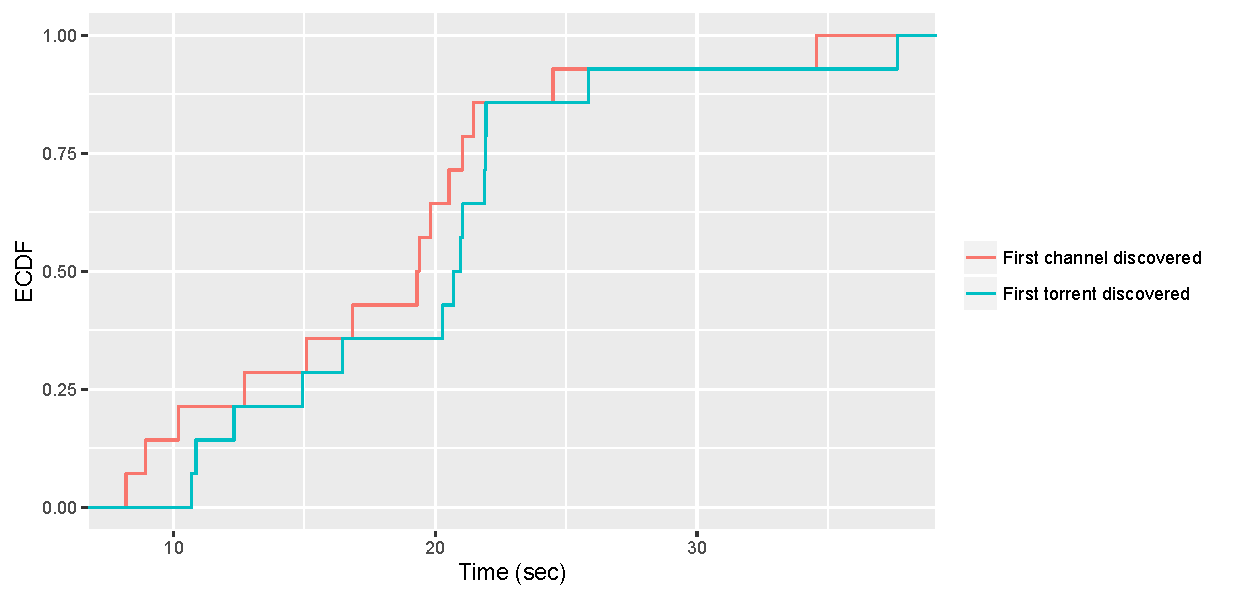
\includegraphics[width=1.0\columnwidth]{images/experiments/content_discovery}
	\caption{The discovery speed of the first channel and torrent after starting Tribler for the first time.}
	\label{fig:content_discovery_speed}
\end{figure}

The delay of discovering the first channel is reasonably: on average, this happens 18 seconds after start-up. In all runs, we have our first channel discovered within 35 seconds. Discovery times of the first torrent is slightly slower and in all runs, the first torrent in a channel is discovered within 40 seconds. Figure \ref{fig:content_discovery_speed} suggests that a torrent discovery always happens after there is at least one discovered channel. This is true: after the channel is discovered, the \emph{PreviewChannel} community is joined where torrents are exchanged and discovered.\\\\
In the old user interface, users were presented with a blank screen with no feedback about new discovered content. In the new interface, the user is presented with a screen that informs the user that Tribler is discovering the first content. This screen is only shown the first time Tribler is started and goes away when there are five discovered channels, after which the page with discovered channels is displayed to the user.

\section{Channel subscription}
When Tribler runs idle, not all available content in the network is discovered. The majority of content is discovered when users subscribe to channel (in the old user interface, this is referenced to as marking a channel as favourite). When Tribler discovers a new channel, users are presented with a preview of this channel. Internally, Tribler connects to the \emph{PreviewChannelCommunity} associated with that channel, a community derived from the \emph{ChannelCommunity}. In this preview community, the amount of torrents that are collected is limited. The \emph{ChannelCommunity} in turn is joined the moment the user subscribes to a channel, after which the full range of content is synchronized. Removing the preview mechanism might significantly increases the resource usage of the Tribler session since the amount of incoming messages to be decoded and verified will increment.\\\\
The experiment as described in this Section, will focus on the discovery speed of additional content after the user subscribes to a specific channel and on the resource allocation when we are running Tribler without enabling a preview mechanism of channels. For the first experiment where we determine the discovery speed of additional content inside a channel, the twenty most popular channels (with the most subscribers) are determined. For this purpose, we are using a Tribler state directory with many discovered channels but void of any channel subscriptions. Exactly ten seconds after Tribler started, we subscribe to one of these popular channels and we measure the interval between subscription to the channel and discovery of the first additional torrent. Tribler is restarted between every run and the state directory is cleaned so we guarantee a clean state of the system. The observed results are visible in Figure \ref{fig:channel_subscription}.

\begin{figure}[!h]
	\centering
	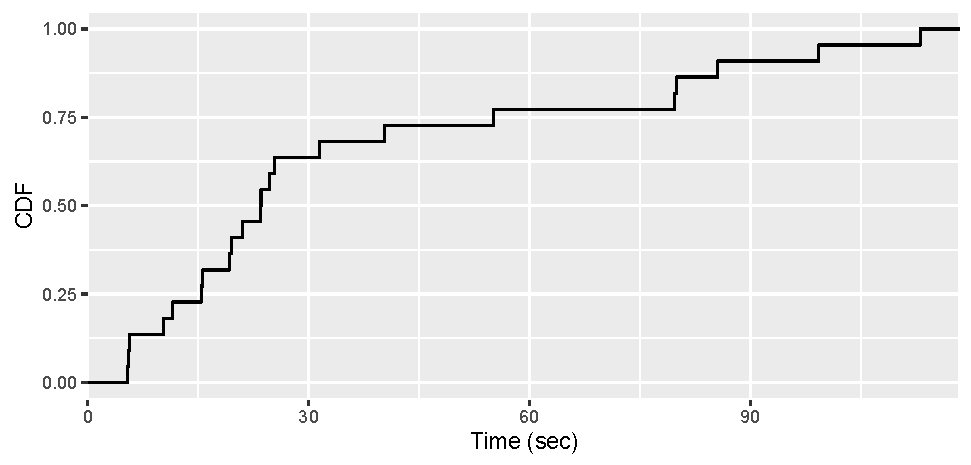
\includegraphics[width=1.0\columnwidth]{images/experiments/channel_subscription}
	\caption{The distribution of discovery times of the first additional torrent after subscribing to a popular channel.}
	\label{fig:channel_subscription}
\end{figure}

The average discovery time of additional torrents after subscription to a channel is 36.8 seconds which is quite long, compared to the discovery speed of the first channel and torrent as described in Section \ref{sec:content-discovery}. The discovery times have a high variation as can be seen in Figure \ref{fig:channel_subscription}. This can be explained by the fact that immediately after subscribing to a channel, Tribler will connect to the \emph{ChannelCommunity} that is joined after subscription and peers have to be found.\\\\
To verify the impact of automatically subscribing to each channel when it is discovered, we perform a CPU usage measurement. In two idle runs of a Tribler session, both lasting for ten minutes, we measure the CPU usage every ten seconds using output provided by the \emph{top} tool. In the first run, a regular Tribler session is used where previews of discovered channels are enabled. In the second run, we bypass the preview of a discovered channel and immediately join the channel, synchronizing all available content. Both types of runs start with an empty state directory. The results of this experiment are visible in Figure \ref{fig:channel_subscription_cpu}.

\begin{figure}[!h]
	\centering
	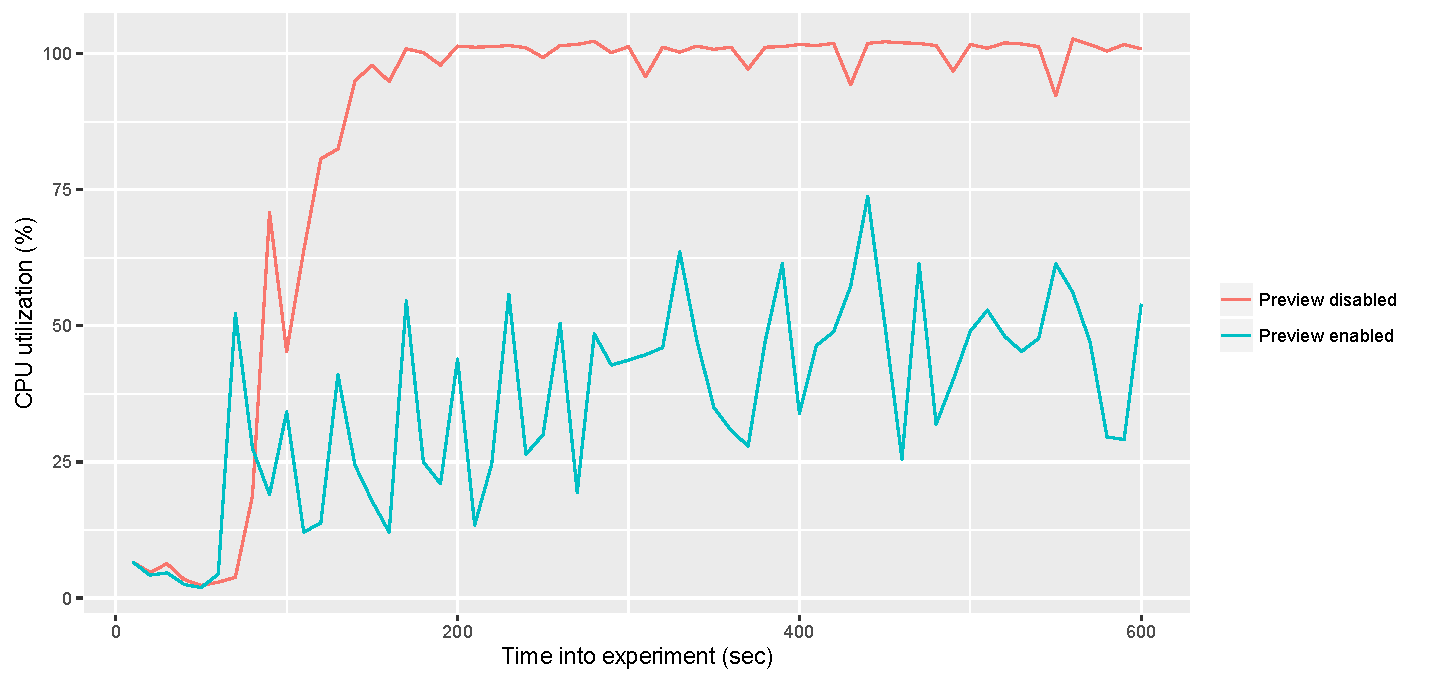
\includegraphics[width=1.0\columnwidth]{images/experiments/subscribe_cpu_experiment}
	\caption{The CPU utilization of one core during a period of ten minutes with channel preview enabled and disabled.}
	\label{fig:channel_subscription_cpu}
\end{figure}

Whereas the CPU usage of the normal run is around 45\% on average, the CPU is busy and quickly rises to 100\% utilization when we enable the auto-join mechanism of channels. This shows that it is infeasible to enable this auto-join feature if we still wish to guarantee a responsive system. One might limit the rate at which discovered torrents are fetched, however, this requires a feedback mechanism where we should notify other peers in the community to limit the amount of messages sent to the peer that is discovering content. Implementing of such as feature is outside the scope of this thesis work and is considered future work.

\section{Torrent Availability and Lookup Performance}
While specific information about torrents such as the name and file names are distributed within the Dispersy communities, this does not hold for the meta info about the torrent itself, which includes additional data such as trackers and piece information. This meta info can be important for users since trackers provides information about the health of a torrent swarm. The experiments as explained in this Section, will investigate the torrent availability and lookup performance of meta info of torrents, either by using downloading them from remote peers in the Tribler network or from the Distributed Hash Table (DHT).

\subsection{TFTP Handler}
When users are performing a remote torrent search, the first three incoming results are pre-fetched which means that the meta info of these torrents are fetched automatically. An incoming search result can possibly contain information about remote peers (candidates) that have the meta info of this torrent available. If candidates for a specific remote torrent result are present, an attempt to fetch the torrent meta info from this candidate is scheduled. This request is performed using the Trivial File Transfer Protocol (TFTP)\cite{sollins1992tftp} which is a simplified version of the more sophisticated File Transfer Protocol (FTP), commonly used to transfer files over the internet. TFTP is also used to transfer meta data about torrent files such as thumbnails between peers, however, meta data of torrents is currently disabled in Tribler. The implementation of TFTP can be found in the core package in the code base.\\\\
There has been no published studies yet about the performance of our TFTP implementation so we have no available reference material. The experiment performed in this Subsection will focus on the performance of TFTP when fetching meta info from remote peers. We start from a clean state directory and exactly one minute after starting Tribler, we perform a remote torrent search. For each incoming remote search result, we perform a TFTP request for each candidate attached to this result. We perform ten remote torrent search operations, with interval of 60 seconds between them. After eleven minutes, we stop Tribler and gather the statistics of the TFTP sessions.\\

\begin{table}[h!]
	\centering
	\begin{tabular}{|l|l|}
		\hline
		\emph{Total requests scheduled} & 1008 \\ \hline
		\emph{Requests in queue} & 761 (75.5\%)\\ \hline
		\emph{Requests failed} & 106 (10.5\%)\\ \hline
		\emph{Requests succeeded} & 141 (14.0\%)\\ \hline
	\end{tabular}
	\caption{A breakdown of the performed requests during the TFTP performance measurement.}
	\label{table:tftp-performance}
\end{table}

We notice that the queue keeps growing: when our experiment is finished, 75.5\% of the initiated requests is still in the queue. The second observation is the high failure rate, when compared to the amount of succeeded requests (42.9\% if we do not consider the requests in the queue). We identified two underlying reasons for the failed requests. Some of the requests timed out, possibly due to the fact that some remote peers are not connectible. A solution for this kind of failure would be a more robust NAT puncturing method. The other reason is that the remote peer does not have the requested file in the local persistent storage. While this situation might seem unusual, it can happen if the remote peer has the requested torrent in the SQLite database but not in the meta info store. We can solve this by not returning this peer as candidate if the torrent is not available in the meta info store. This solution will also reduce the total bandwidth used by the TFTP component.\\\\
Next, we will focus on the turnaround time of the successful TFTP requests, these are displayed in figure \ref{fig:tftp_performance} in an ECDF. Here, we notice the weird distribution of the turnaround times. We would expect that the total request times to fetch torrents is somewhat constant, however, we see outgoing requests that take over 400 seconds to complete. This trend will probably continue if we did not stop the experiment after ten minutes. The most logical explanation for this is that requests are added to the request queue at a faster rate than the processing speed of these requests. This also explains the values denoted in Table \ref{table:tftp-performance} where 75.5\% of the request are still in the queue after the experiment ends. Better support for parallel requests should help, however, this is considered further work and outside the scope of this thesis work.

\begin{figure}[!h]
	\centering
	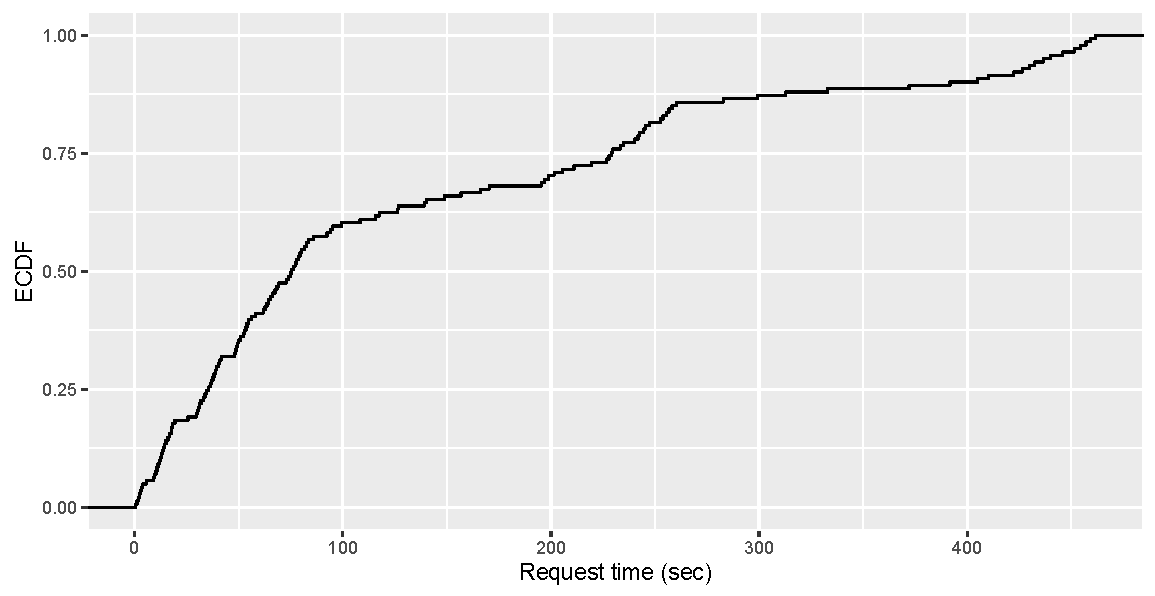
\includegraphics[width=0.9\columnwidth]{images/experiments/tftp_performance}
	\caption{An ECDF of the performance of the torrent meta info download mechanism using TFTP in Tribler.}
	\label{fig:tftp_performance}
\end{figure}

\subsection{Distributed Hash Table}
A\todo{CDF niet tot 1 laten lopen} possible source of torrents is the Distributed Hash Table (DHT). The DHT provides primitives to query torrent files and peers, based on a specific infohash of a torrent. Querying the DHT for torrent files can be done by invoking the \emph{download\_torrentfile} in the \emph{Session} object. One should specify the callback to be invoked after the meta info is successfully downloaded. In this Section, experiments will be conducted to get insights in the availability of torrent files and the performance of lookup operations in the DHT. This experiment is has a relevance to user experience since users that want to determine whether specific content is interesting or not, they first might want to view meta info of the torrent file, such as names and sizes of the files. This meta info should be available as soon as possible.\\\\
In the current user interface, the torrent file is fetched when the user single clicks on a torrent in the list of torrents, either when browsing through contents of a channel or after performing a remote keyword search. In addition, when executing a remote search, the first three top-results are pre-fetched since the user might be interested in them. For this experiment, a popular channel with over 5.000 torrents is considered and a subset of torrent infohashes in this channel is taken. Every 40 seconds, a DHT query is performed with one of the 1.000 random infohashes. The time-out period used in Tribler is 30 seconds, after which a failure callback is invoked and an error is displayed in the user interface to notify the user about the failed request. The results of this experiments are visible in Figure \ref{fig:metainfo_fetch}. Torrents that cannot be successfully resolved from the DHT, are assigned a value of 30 seconds in the graph.\\

\begin{figure}[!h]
	\centering
	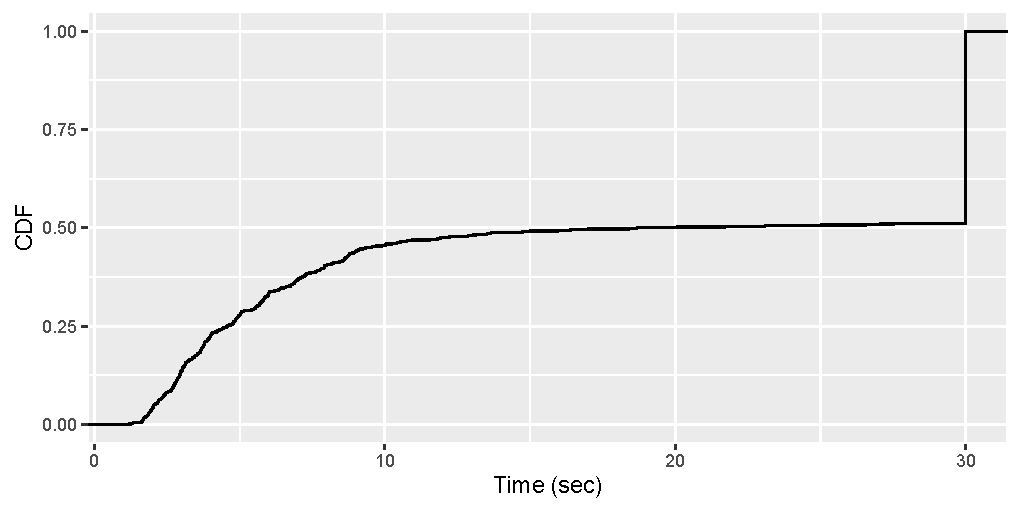
\includegraphics[width=0.9\columnwidth]{images/experiments/metainfo_fetch}
	\caption{Test.}
	\label{fig:metainfo_fetch}
\end{figure}

We immediately notice that the failure rate of DHT lookups is quite high: a little under 50\% of the lookup operations are timing out. This issue might be addressed to dead torrents (when no peers in the DHT have this torrent information available) or private torrents (torrents which information is not available in the DHT). The amount of failures might be even higher in a less popular channel since the content in these channels are probably less seeded. As explained in the previous Subsection, the DHT is not the only source for torrents in Tribler and we might also fetch torrents from other peers using TFTP. Unfortunately, the approach of fetching meta info about torrents from other peers is only usable when searching for torrents. Caching and exchanging torrent candidates is not successful since the availability of candidates cannot be guaranteed.\\\\
The average lookup time of torrents that are successfully fetched from the DHT is 5.81 seconds which is reasonably fast. Additionally, Figure \ref{fig:metainfo_fetch} shows that a little over 90\% of the successfully fetched torrents are retrieved within 10 seconds.\\\\
To improve performance of metainfo lookup, dead torrents should be handled correctly. One possible solution might be an implementation of a periodical check for each incoming torrent. By limiting the number of outstanding DHT requests, this approach does not create require much additional resources. To further improve performance, the result of DHT lookups might be disseminated to remote peers in the network. Torrents that are not successfully fetched from the DHT, could be hidden automatically in the user interface. The downside of this approach is that it might not give a realistic view of the availability of a torrent since their might be candidates which have a copy of this torrent available.